\documentclass{beamer}
%\usetheme{Ilmenau}
%\usecolortheme{beaver}

\usepackage[slovak,american]{babel}
\usepackage[utf8]{inputenc}
\usepackage{graphicx}
\usepackage{adjustbox}
\usepackage{xcolor}
\usepackage{mathrsfs}
 
 \newsavebox\MBox
\newcommand\Cline[2][red]{{\sbox\MBox{$#2$}%
  \rlap{\usebox\MBox}\color{#1}\rule[-2.2\dp\MBox]{\wd\MBox}{1pt}}}

%\usefonttheme{serif}

%\definecolor{UKOrange}{HTML}{ef9424} %
\definecolor{UKOrange}{HTML}{7a2c18} %
\definecolor{UKBrown}{HTML}{a96d5e} %
\definecolor{UKLight}{HTML}{d8b6ab} %
\definecolor{UKDark}{HTML}{7a4f44}
\definecolor{UKDarker}{HTML}{4d312b} 
\definecolor{UKDarkest}{HTML}{2e1e1a}
\definecolor{UKRed}{HTML}{bf1f1c}

\setbeamertemplate{footline}[frame number]{}
\setbeamertemplate{navigation symbols}{}

%\usecolortheme{beaver}
\setbeamertemplate{itemize item}[square]
\setbeamercolor{itemize item}{fg = UKBrown}
\setbeamercolor{itemize subitem}{fg = UKLight}
\setbeamercolor{enumerate item}{fg = UKDark}

\setbeamercolor{footnote}{fg=UKLight}
\setbeamercolor{footnote mark}{fg=UKLight}
\setbeamerfont{footnote}{size=\tiny}
\renewcommand\footnoterule{}

\usetheme{default}
\beamertemplatenavigationsymbolsempty
\setbeamercolor{title}{fg=white, bg=UKBrown}
\setbeamercolor{frametitle}{fg=white, bg=UKBrown}
\setbeamercolor{block title}{bg=UKBrown, fg= white}
\setbeamercolor{block body}{bg =UKLight, fg = UKDarkest}

\setbeamercolor{block title alerted}{bg=UKOrange, fg= white}
\setbeamercolor{block body alerted}{bg =UKLight, fg = UKDarkest}


%\setbeamercolor{section in toc}{fg = UKBrown}
%\setbeamercolor{section in toc}{fg = UKDarkest}

% odstrani gulicky
\renewcommand*{\slideentry}[6]{}

\useoutertheme[subsection=false]{miniframes}
\AtBeginSection[]{\subsection{}}

\setbeamercolor{below lower separation line head}{bg=UKDark}
\addtobeamertemplate{headline}{}{%
  \begin{beamercolorbox}[colsep=0.5pt]{below lower separation line head}
  \end{beamercolorbox}
}
%\setbeamercolor*{mini frame}{fg=white,bg=UKRosy}
\setbeamercolor{section in head/foot}{fg=UKLight, bg=UKDark}

\usepackage{etoolbox}
\makeatletter
\preto{\@verbatim}{\topsep=0pt \partopsep=0pt }
\makeatother

%\setbeamertemplate{itemize/enumerate body begin}{\normalsize}
%\setbeamertemplate{itemize/enumerate subbody begin}{\normalsize}




%\newcommand{\codeblock}[2]{ \begin{block}{#1} \begin{verbatim}#2\end{verbatim}\end{block}}

%\defbeamertemplate*{title page}{customized}[1][]
%{
%  \begin{centering}
%    \begin{beamercolorbox}[sep=8pt,center]{title}
%      \usebeamerfont{title}\inserttitle
%    \end{beamercolorbox}
%  \end{centering}
%  \bigskip
%
%\begin{columns}[onlytextwidth,T]
%
%
%  \column{27mm}
%  \includegraphics[width=27mm]{images/logoFMFI.png}
%  
%  \column{\dimexpr\linewidth-54mm-6mm}
%  \centering
%  \vspace{5mm}  
%  \usebeamerfont{author}\insertauthor\par
%  \vspace{5mm}
%  \usebeamerfont{institute}\insertinstitute\par
%
%  \column{27mm}
%  \includegraphics[width=27mm]{images/logoUK.png}  
%\end{columns}
%\centering
%\vspace{7mm}
%  \usebeamerfont{date}\insertdate\par
%}

\DeclareMathOperator*{\argmin}{arg\,min}
\newcommand{\e}[1]{$\cdot 10^{#1}$}

%\newcommand{\codeblock}[2]{ \begin{block}{#1} \begin{verbatim}#2\end{verbatim}\end{block}}



\title[10. cvičenie]{Advanced Image Processing - Segmentation}
\author[Kocur]{Ing. Viktor Kocur \\{\small viktor.kocur@fmph.uniba.sk}}
\institute{DAI FMFI UK}
\date{27.11.2017}

\begin{document}
\selectlanguage{slovak}


\begin{frame}

  \titlepage

\end{frame}

\section{Segmentation}
\subsection{What is segmentation}

\begin{frame}
\frametitle{Goal of segmentation}
\begin{block}{Goal of segmentation}
The goal of segmentation is to divide the image into disjunct areas so that the areas correspond to singular objects.
\end{block}

\begin{block}{Partial segmentation}
It is not always necessary to segment the image into all objects. Sometimes a partial segmentation is sufficient. In that case only one or more objects can be segmented.

\end{block}
\end{frame}

\begin{frame}
\frametitle{Original Image}
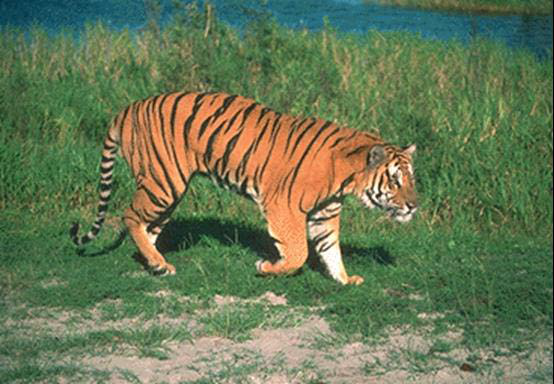
\includegraphics[width=\textwidth]{tiger.png}
\end{frame}

\begin{frame}
\frametitle{Segmented Image}
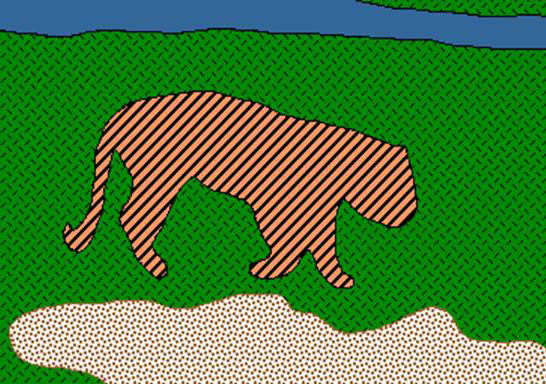
\includegraphics[width=\textwidth]{tiger_segmented.png}
\end{frame}



\section{k-means clustering}

\subsection{Algoritmus}

\begin{frame}
\frametitle{k-means clustering}

\begin{block}{k-means}
k-means clustering is a method which clusters points into k groups
\end{block}

\begin{block}{Postup}
\begin{itemize}
\item In the given vector space place k random centroids
\item For each point in the space determine the closest centroid
\item Move the centroids so that they are now in the center of their corresponding poitns
\item Repeat step 2 and 3 until the centroids no longer move
\end{itemize}
\end{block}
\end{frame}

\begin{frame}
\frametitle{k-means}
\begin{center}
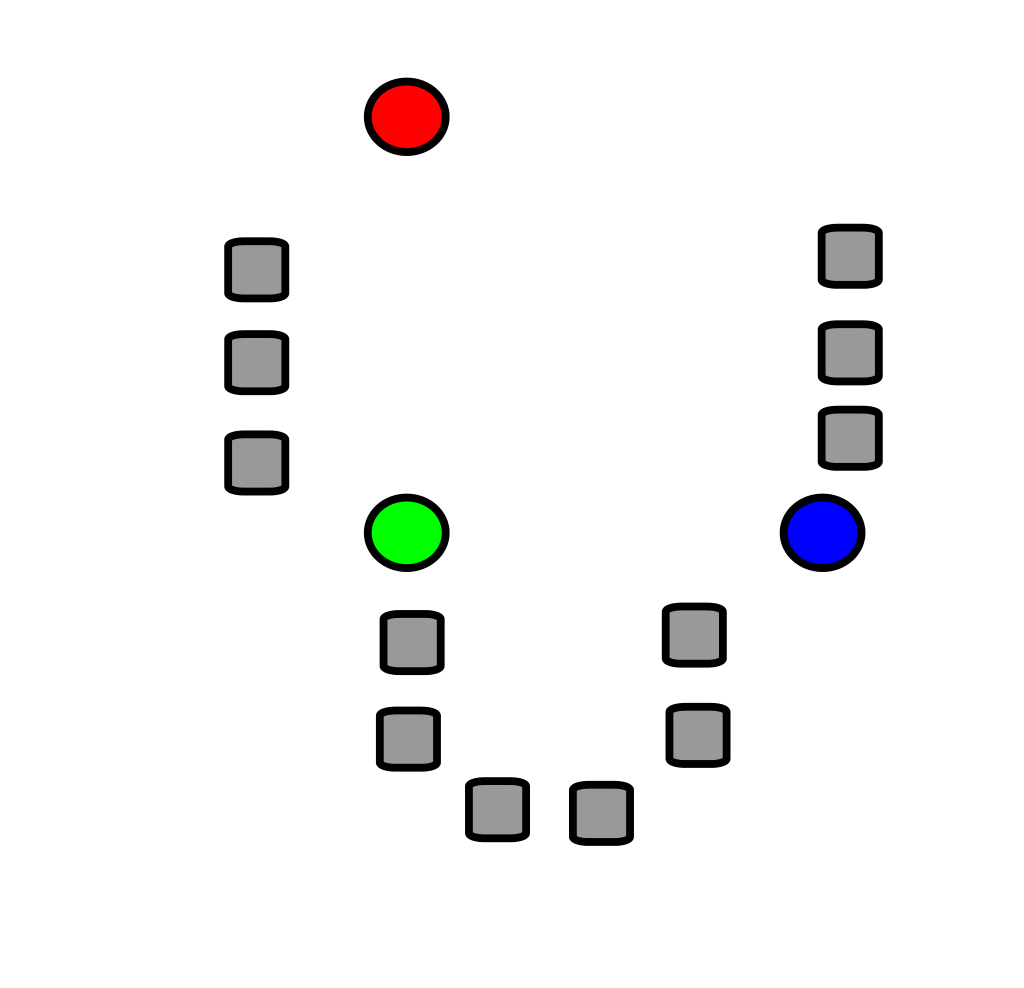
\includegraphics[width=0.8\textwidth]{km1.png}
\end{center}
\end{frame}

\begin{frame}
\frametitle{k-means}
\begin{center}
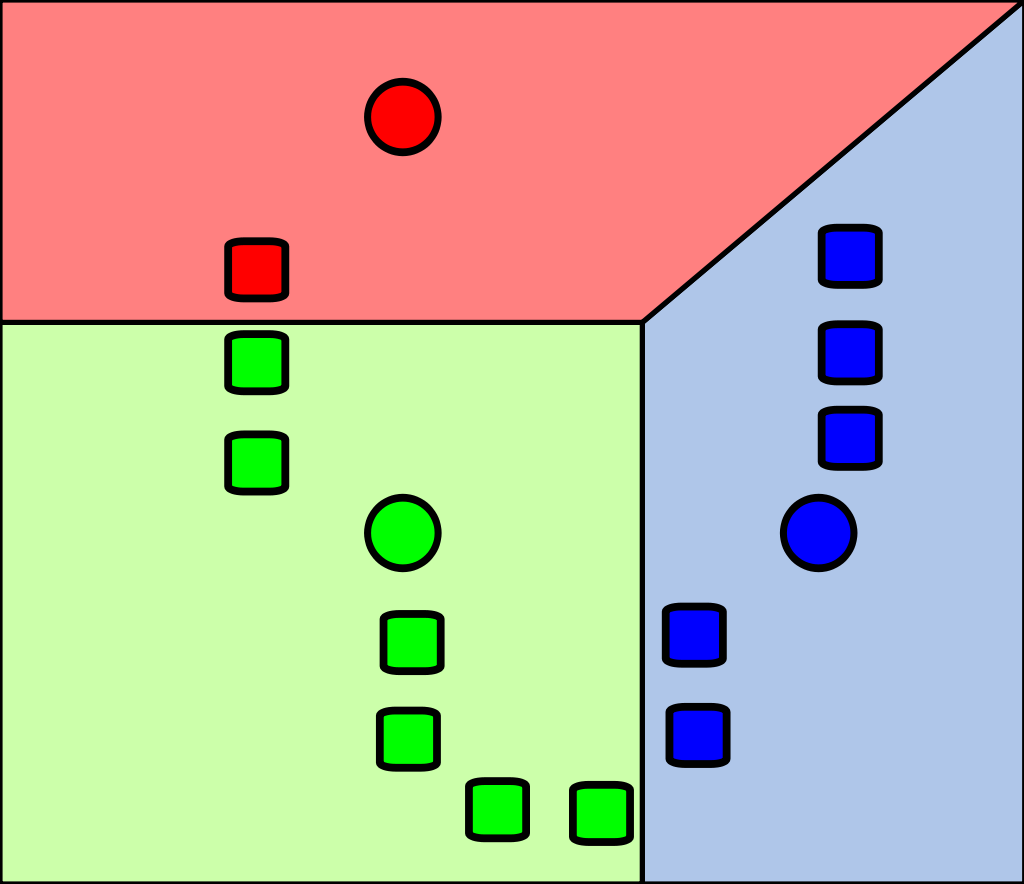
\includegraphics[width=0.8\textwidth]{km2.png}
\end{center}
\end{frame}

\begin{frame}
\frametitle{k-means}
\begin{center}
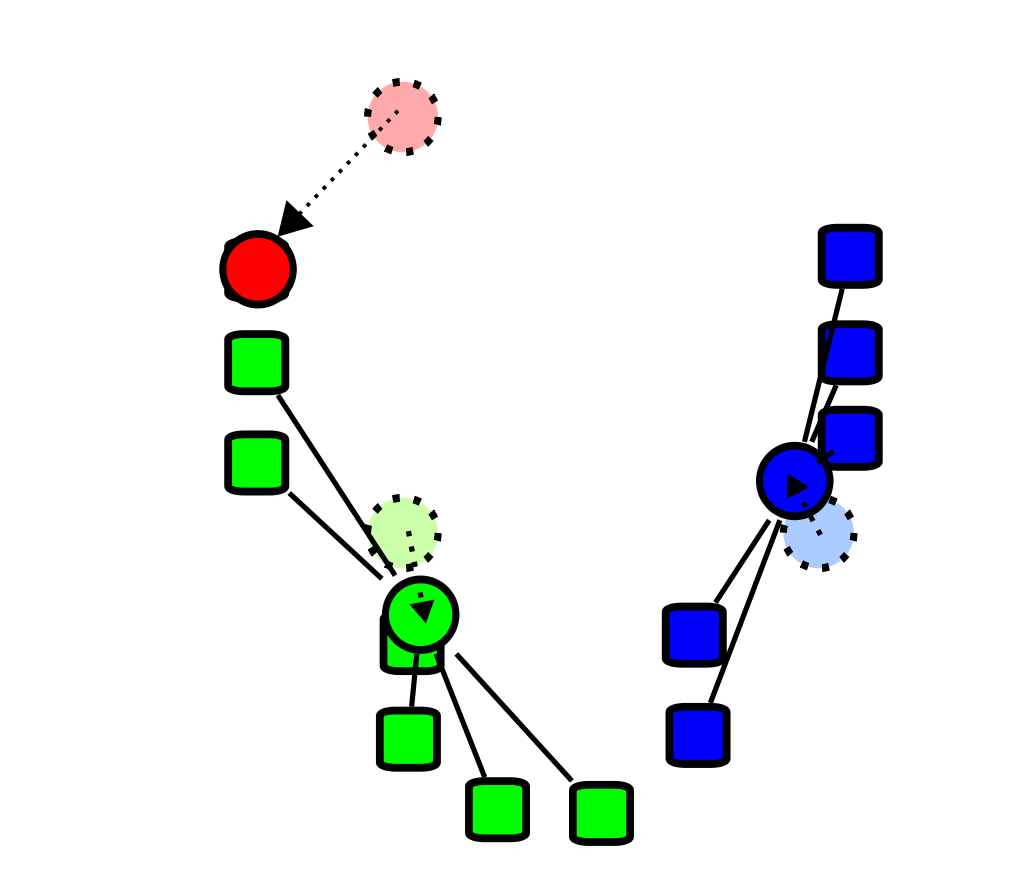
\includegraphics[width=0.8\textwidth]{km3.png}
\end{center}
\end{frame}

\begin{frame}
\frametitle{k-means}
\begin{center}
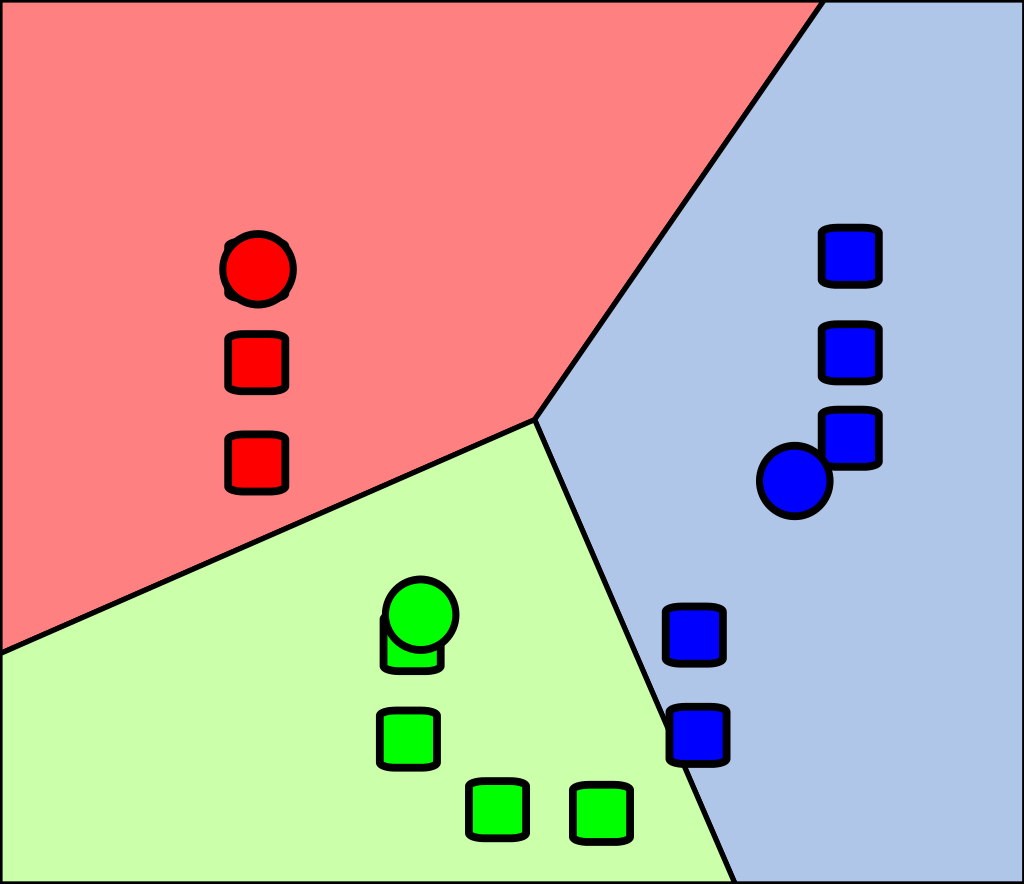
\includegraphics[width=0.8\textwidth]{km4.png}
\end{center}
\end{frame}

\subsection{k-means in Matlab}

\begin{frame}
\frametitle{k-means in matlab}
\begin{block}{kmeans}
kmeans(A, k) - for A matrix with n rows, each of which is one vector in our vector space return a vector of size n with values 1 to k according to the cluster to which each vector corresponds.
\end{block}

\begin{block}{Vectors for image segmentation}
For images we can segment the pixels. The vector space can be represented with color and position of the images.
\end{block}
\end{frame}

\begin{frame}
\frametitle{k-means in matlab}
\begin{block}{Exercise}
Use k-means for zatisie. Use Lab color space for segmentation.
\end{block}

\begin{block}{Exercise}
Add x and y coordinates to the vector space. Do not forget to normalize the components.
\end{block}


\begin{block}{meshgrid}
[X, Y] = meshgrid(1:c,1:r) - creates two matrices of size $r \times c$. X contains the x coordinates and Y contains the y coordinates.

\end{block}
\end{frame}

\section{Color-based Segmentation}

\section{Graph Cut}
\subsection{Graph Cut}

\begin{frame}
\frametitle{Graph Cut}
\begin{block}{Graph Cut}
Graph Cut is a method that uses user input to segment the foreground. User selects a few pixels as the foreground and some as background.
\end{block}

\begin{block}{Algorithm}
A graph containing all pixels is constructed. Each pixel is connected to its neighbors with a weight that corresponds to the pixel similarity. There are two additional nodes in the graph representing the foreground and the background. These are connected to the pixels with a probability based on a distribution of colors selected by the user. In the final step the algorithm cuts a graph so that it minimizes energy, which is calculated using the weights of edges in the graph.
\end{block}

\end{frame}

\begin{frame}
\frametitle{Graph Cut}
\begin{block}{Matlab}
You can use Graph Cut in matlab. Look for image segmenter in the APP context menu.
\end{block}
\end{frame}

\section{Color-based Segmentation}

\begin{frame}
\frametitle{Color-based Segmentation}
\begin{block}{Using user input}
We can also use user input to pick a color in the image and segment pixels based on their distance to the color in some colospace. We can then threshold the distance image to obtain the segmentation.
\end{block}

\begin{block}{Pixel position}
We can also use user input position of the object to also use the spatial information as we did with the k-means clustering.
\end{block}

\begin{block}{Exercise}
Try to use this approach to segment the apples or the orange in the image zatisie. Try different color spaces. Try it without spatial information and with it. Use smoothing and morphological operations to refine the segmentation. 
\end{block}
\end{frame}

\end{document}


\section{Watershed}
\subsection{Watershed}

\begin{frame}
\frametitle{Watershed}
\begin{block}{Watershed}
Watershed method takes image as a topographical map and separates in a manner similar to drainage basins on a map.
\end{block}

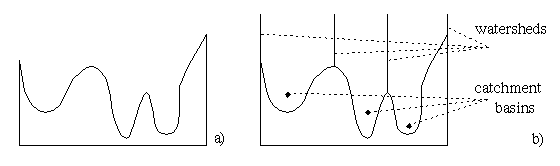
\includegraphics[width=\textwidth]{basins.png}

\begin{block}{Input for watershed}
Watershed is a nice algorithm, but it is first necessary to find an adequate image to obtain the basins.
\end{block}
\end{frame}

\begin{frame}
\frametitle{Po}

\begin{block}{imgradient}
imgradient(I) - returns gradient of a grayscale image
\end{block}

\begin{block}{watershed}
watershed(I) - returns a label matrix after applying watershed algorithm
\end{block}

\begin{block}{label2rgb}
label2rgb(L) - creates a color image with each label having different color
\end{block}

\begin{block}{Úloha}
Load the image pears.png and show its gradient.
\end{block}

\end{frame}


\subsection{Postup}

\begin{frame}
\frametitle{Postup}
\begin{block}{Postup rozdelíme na časti}
\begin{itemize}
\item Otvorenie a zatvorenie pomocou imreconstruct
\item Nájdenie masky popredia
\item Nájdenie hrebeňov v obraze
\item Vynútenie miním na maske
\item Watershed
\end{itemize}
\end{block}

\begin{block}{Link}
Tento postup je aj na stránke: https://www.mathworks.com/help/images/marker-controlled-watershed-segmentation.html
\end{block}
\end{frame}

\begin{frame}[fragile]
\frametitle{Otvorenie a zatvorenie}
\begin{block}{Kód}
\begin{verbatim}
se = strel('disk',20);
Ioc = imclose(imopen(I,se),se);
Ie = imerode(I,se);
Iobr = imreconstruct(Ie,I);
Iobrd = imdilate(Iobr,se);
Iobrcbr = imreconstruct(imcomplement(Iobrd), ...
    imcomplement(Iobr));
Iobrcbr = imcomplement(Iobrcbr);
\end{verbatim}
\end{block}

\begin{block}{Čo sa udialo}
Realizovali sme operáciu otvorenia a následného zatvorenia, ale za použitia markerov, tj pomocou rekonštrukcie.
\end{block}
\end{frame}

\begin{frame}[fragile]
\frametitle{Otvorenie a zatvorenie}
\begin{block}{Kód}
\begin{verbatim}
fgm = imregionalmax(Iobrcbr);
se2 = strel(ones(5,5));
fgm2 = imclose(fgm,se2);
fgm3 = imerode(fgm2,se2);
fgm4 = bwareaopen(fgm3,20);
\end{verbatim}
\end{block}

\begin{block}{Čo sa udialo}
Vytvorili sme masku popredia z oblastí ktoré sú lokálnymi maximami. Potom sme ju pomocou morfológie upravili a nakoniec sme odstránili oblasti s obsahom menším ako 20 pixelov. 
\end{block}
\end{frame}

\begin{frame}[fragile]
\frametitle{Nájdenie hrebeňov pozadia}
\begin{block}{Kód}
\begin{verbatim}
dist = bwdist(imbinarize(Iobrcbr));
ws1 = watershed(dist);
bgm = ws1 == 0;
\end{verbatim}
\end{block}

\begin{block}{Čo sa udialo}
Zobrali sme širšie popredie a pomocou funkcie bwdistance, sme spočítali pre každý pixel vzdialenosť od najbližšieho pixelu popredia. Na tieto vzdialenosti sme aplikovali watershed a získali sme tak oblasti ktoré sú hrebeňmi.
\end{block}
\end{frame}

\begin{frame}[fragile]
\frametitle{Vynútenie minima a watershed}
\begin{block}{Kód}
\begin{verbatim}
grad = imgradient(I);
grad2 = imimposemin(grad, bgm | fgm4);
L = watershed(grad2);
\end{verbatim}
\end{block}

\begin{block}{Čo sa udialo}
Spojili sme masku miest kde chcme mať 'kotliny' a vynútili sme aby na gradientnom obraze boli lokálne minimá len tam. Týmto spôsobom sa samostatne segmentujú objekty a zároveň aj pozadie bude mať svoje povodie. Nakoniec aplikujeme watershed.
\end{block}
\end{frame}

\begin{frame}[fragile]
\frametitle{Krajšie zobrazenie obrázka}
\begin{block}{Kód}
\begin{verbatim}
figure
imshow(I)
hold on
himage = imshow(Lrgb);
himage.AlphaData = 0.3;
\end{verbatim}
\end{block}

\begin{block}{Čo sa udialo}
Len sme vykreslil obrázok pekným spôsobom.
\end{block}
\end{frame}
